% !TeX root = ..\main.tex
\section{Thiết kế cơ sở dữ liệu}
\par Nhóm lựa chọn kiến trúc Microservice cho hệ thống, với việc chia ra các service nhỏ và mỗi service có một database riêng phục vụ cho nghiệp vụ của riêng service đó, nên ở đây các database được thiết kế riêng lẻ cho từng service.

\subsection{ERD/EERD}
\subsubsection{Service Hàng hóa}
\begin{figure}[!htp]
    \begin{center}
        \includegraphics[width=1\textwidth]{img/database/erd/shop_online-hàng.png}
        \newline
        \caption{ERD cho database của service Hàng hóa}
    \end{center}
\end{figure}

\par Database của service Hàng hóa bao gồm hai thực thể là Hàng hóa và Hàng trong kho. Thực thể hàng hóa chỉ thông tin các mặt hàng được bán, bao gồm các thuộc tính:
\begin{itemize}
    \item Mã hàng: thuộc tính khóa, là mã của mặt hàng.
    \item Kích thước: thuộc tính khóa, là kích thước của mặt hàng.
    \item Màu: thuộc tính khóa, là màu của mặt hàng.
    \item Tên hàng: là tên của mặt hàng.
    \item Lứa tuổi: là lứa tuổi phù hợp của mặt hàng.
    \item Giới tính: là giới tính phù hợp của mặt hàng.
    \item Nhà sản xuất: là nhà sản xuất của mặt hàng.
    \item Hình ảnh: thuộc tính đa trị, bao gồm các hình ảnh của mặt hàng.
    \item Được bán: cho biết mặt hàng có đang được mở bán hay không.
    \item Đơn giá: giá tiền cho một đơn vị của mặt hàng.
    \item Mô tả: thông tin thêm về mặt hàng.
    \item Loại: thể loại của mặt hàng.
    \item Số lượng hiện tại: thuộc tính dẫn xuất, là số lượng còn tồn hiện tại của mặt hàng.
\end{itemize}

\par Thực thể Hàng trong kho chỉ thông tin của mặt hàng trong một kho nào đó. Thực thể này bao gồm các thuộc tính:
\begin{itemize}
    \item Mã kho: thuộc tính khóa, là mã của kho chứa hàng đó.
    \item Số lượng: số lượng hàng đó còn trong kho.
    \item Ngày tạo: ngày mặt hàng lần đầu vào kho.
    \item Ngày thay đổi: ngày hàng trong kho có sự thay đổi.
\end{itemize}

\par Hàng hóa và Hàng trong kho có mối quan hệ Bao gồm, đây là mối quan hệ bắt buộc, 1-N: hàng hóa bắt buộc phải nằm trong kho, và một mặt hàng có thể nằm ở nhiều kho; hàng trong kho bắt buộc thuộc về một mặt hàng, và chỉ thuộc về duy nhất một mặt hàng.

\subsubsection{Service Đơn hàng}
\begin{figure}[!htp]
    \begin{center}
        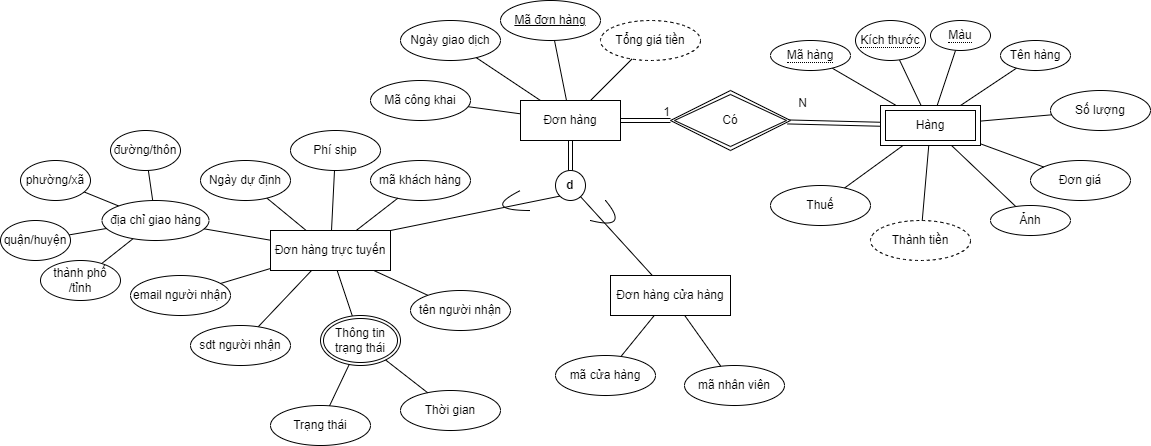
\includegraphics[width=1\textwidth]{img/database/erd/shop_online-đơnhàng.png}
        \newline
        \caption{ERD cho database của service Đơn hàng}
    \end{center}
\end{figure}

\par Database của service Đơn hàng bao gồm các thực thể Đơn hàng và Hàng hóa, chỉ các hàng hóa trong đơn hàng. Đơn hàng được cụ thể hóa xuống Đơn hàng online và Đơn hàng cửa hàng.
\par Thực thể Đơn hàng gồm các thuộc tính:
\begin{itemize}
    \item Mã đơn hàng: thuộc tính khóa, chỉ mã của đơn hàng.
    \item Ngày giao dịch: ngày thực hiện giao dịch mua hàng và sinh ra đơn hàng.
    \item Tổng giá tiền: thuộc tính dẫn xuất, là tổng giá tiền của đơn hàng.
\end{itemize}

\par Thực thể Đơn hàng online có thêm các thuộc tính:
\begin{itemize}
    \item Mã khách hàng: là mã khách hàng đã mua hàng online.
    \item Phí ship: giá tiền cho việc vận chuyển đơn hàng.
    \item Mong đợi: ngày giao hàng mong đợi.
    \item Thông tin trạng thái: thuộc tính phức hợp, bao gồm các thông tin Trạng thái và Thời gian chỉ các trạng thái và thời gian đạt đến trạng thái đó của đơn hàng.
\end{itemize}

\par Thực thể Đơn hàng cửa hàng có thêm thuộc tính:
\begin{itemize}
    \item Mã cửa hàng: mã cửa hàng bán hàng trong đơn hàng.
\end{itemize}

\par Thực thể Hàng bao gồm các thuộc tính:
\begin{itemize}
    \item Mã hàng: thuộc tính khóa, là mã của mặt hàng trong đơn hàng.
    \item Kích thước: thuộc tính khóa, là kích thước của hàng trong đơn hàng.
    \item Màu: thuộc tính khóa, là màu của hàng trong đơn hàng.
    \item Số lượng: số lượng hàng đã mua trong đơn hàng.
    \item Đơn giá: giá tiền một đơn vị của hàng trong đơn hàng.
    \item Thuế: giá tiền thuế của hàng trong đơn hàng.
    \item Thành tiền: thuộc tính dẫn xuất, là tổng giá tiền (đơn giá * số lượng) + thuế.
\end{itemize}

\par Đơn hàng và Hàng có quan hệ Bao gồm, đây là quan hệ bắt buộc, 1-N: đơn hàng bắt buộc có hàng, và có thể có nhiều hàng; hàng trong đơn hàng bắt buộc phải thuộc về một mặt hàng, và chỉ thuộc về duy nhất một mặt hàng.

\subsubsection{Service Kho}
\begin{figure}[!htp]
    \begin{center}
        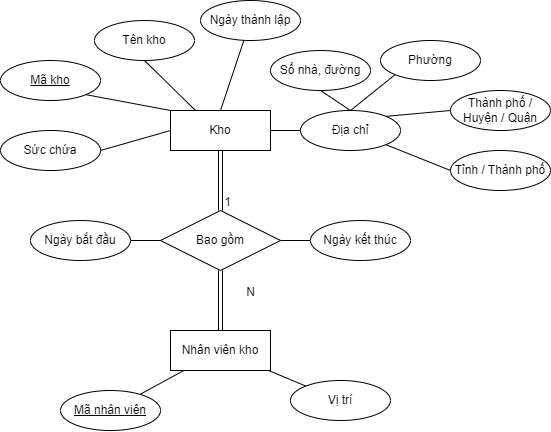
\includegraphics[width=1\textwidth]{img/database/erd/shop_online-Kho.png}
        \newline
        \caption{ERD cho database của service Kho}
    \end{center}
\end{figure}

\par Database của service Kho bao gồm thực thể Kho và thực thể Nhân viên kho. Thực thể Kho bao gồm các thuộc tính:
\begin{itemize}
    \item Mã kho: thuộc tính khóa, là mã của kho.
    \item Tên kho: tên của kho.
    \item Ngày thành lập: ngày mà kho đi vào sử dụng.
    \item Địa chỉ: thuộc tính kết hợp, bao gồm các thuộc tính Số nhà, đường, Phường, Thành phố / Quận / Huyện, Tỉnh / Thành phố.
    \item Sức chứa: sức chứa hàng tối đa của kho.
    \item Còn lại: thuộc tính dẫn xuất, chỉ sức chứa còn lại mà kho có thể chứa hàng thêm.
\end{itemize}

\par Thực thể Nhân viên kho bao gồm các thuộc tính:
\begin{itemize}
    \item Mã nhân viên: thuộc tính khóa, là mã của nhân viên làm việc ở kho.
\end{itemize}

\par Kho và nhân viên kho có mối quan hệ Bao gồm là mối quan hệ bắt buộc, M-N: kho bắt buộc có nhân viên, và có thể có nhiều nhân viên làm việc; nhân viên buộc phải làm việc ở ít nhất một kho, và có thể làm việc ở nhiều kho. Mối quan hệ này có các thuộc tính:
\begin{itemize}
    \item Ngày bắt đầu: ngày nhân viên bắt đầu làm việc tại kho đó.
    \item Ngày kết thúc: ngày nhân viên nghỉ làm việc tại kho đó.
\end{itemize}

\par Mỗi kho có một quản lý, nên kho và nhân viên quản lý có mối quan hệ Được quản lý bởi. Mối quan hệ là M-N. Kho tham gia vào mối quan hệ với ràng buộc tham gia bắt buộc: kho phải có quản lý, và theo thời gian có nhiều quản lý theo từng thời gian khác nhau. Quản lý - cũng là nhân viên kho, tham gia vào mối quan hệ với ràng buộc tham gia không bắt buộc, một nhân viên không cần phải làm quản lý, và qua thời gian có thể làm quản lý ở nhiều kho. Mối quan hệ này có các thuộc tính:
\begin{itemize}
    \item Ngày bắt đầu: ngày quản lý bắt đầu làm việc tại kho đó.
    \item Ngày kết thúc: ngày quản lý nghỉ làm việc tại kho đó.
\end{itemize}

\subsection{Ánh xạ}
\par Từ các ERD/EERD trên, chúng ta có các ánh xạ sau tương ứng với mỗi service.

\subsubsection{Service Hàng hóa}
\begin{figure}[!htp]
    \begin{center}
        \includegraphics[width=1\textwidth]{img/database/mapping/mapping-hàng.png}
        \newline
        \caption{Ánh xạ cho database của service Hàng hóa}
    \end{center}
\end{figure}

\subsubsection{Service Đơn hàng}
\begin{figure}[!htp]
    \begin{center}
        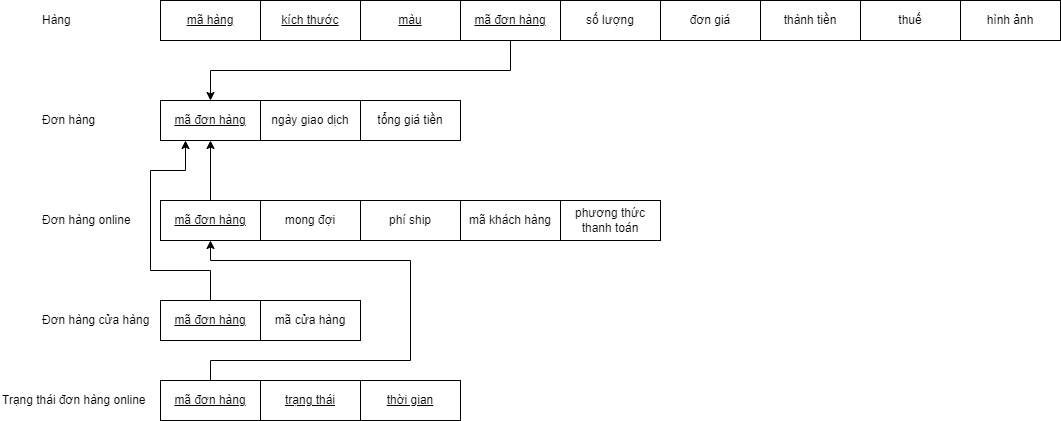
\includegraphics[width=1\textwidth]{img/database/mapping/mapping-đơnhàng.png}
        \newline
        \caption{Ánh xạ cho database của service Đơn hàng}
    \end{center}
\end{figure}

\subsubsection{Service Kho}
\begin{figure}[!htp]
    \begin{center}
        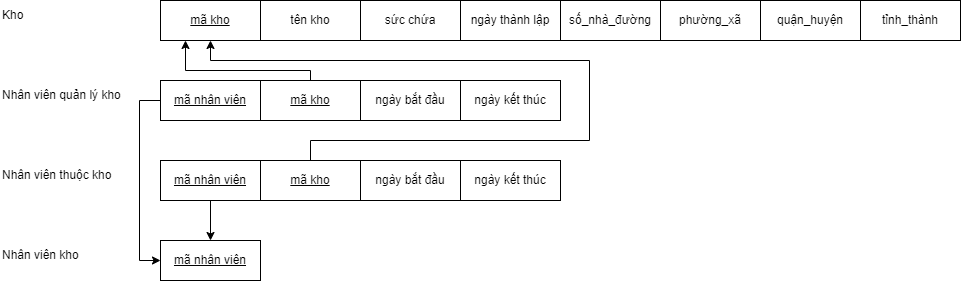
\includegraphics[width=1\textwidth]{img/database/mapping/mapping-kho.png}
        \newline
        \caption{Ánh xạ cho database của service Kho}
    \end{center}
\end{figure}